\documentclass[12pt]{article}
\usepackage[top=0.5in,bottom=0.25in,left=0.75in,right=0.75in]{geometry}

\usepackage{amssymb,amsmath,graphicx,multicol}

\usepackage[export]{adjustbox}
\newcommand{\I}{\phantom{\scalebox{1.5}[1]{$\displaystyle \sum_x^y$}}}
\newcommand{\tallspace}{\phantom{\scalebox{0.01}[1]{$\displaystyle \sum_x^y$}}}

%\newcommand{\ds}{\displaystyle}

\setlength{\topmargin}{-.9in}
\setlength{\textwidth}{6.8in}
\setlength{\textheight}{9.3in}
\setlength{\oddsidemargin}{-.2in}
\setlength{\evensidemargin}{-.2in}

\pagestyle{empty}
\begin{document}


{\sc \noindent Transformations, Even/Odd Functions, Inverses, Composition (1.3) \hfill Math 115}  \hrule

%Note to instructors: not all the transformations are represented here, so you might want to point out those that are not, i.e. vertical stretches, and horizontal reflection.  
%
%It's also really helpful to point out that vertical transformations are achieved by doing an operation to the output, while horizontal transformations are achieved by replacing the input by some something new.

\begin{minipage}[t][][c]{0.5\textwidth}
	
	\bigskip
	
	$$\begin{array}{|c|c|c|c|c|} \hline
	x  & -1 & 0 & 1 & 3 \\ \hline
	f(x)  & 2  & -1 & -2  & 2  \\
	\hline
	\end{array}$$	
	
	Use the graph provided for $f(x)$ to sketch the graph and fill in some values of the table for some of the related functions below.
	%Verbal description: This is the u
\end{minipage} \hfill 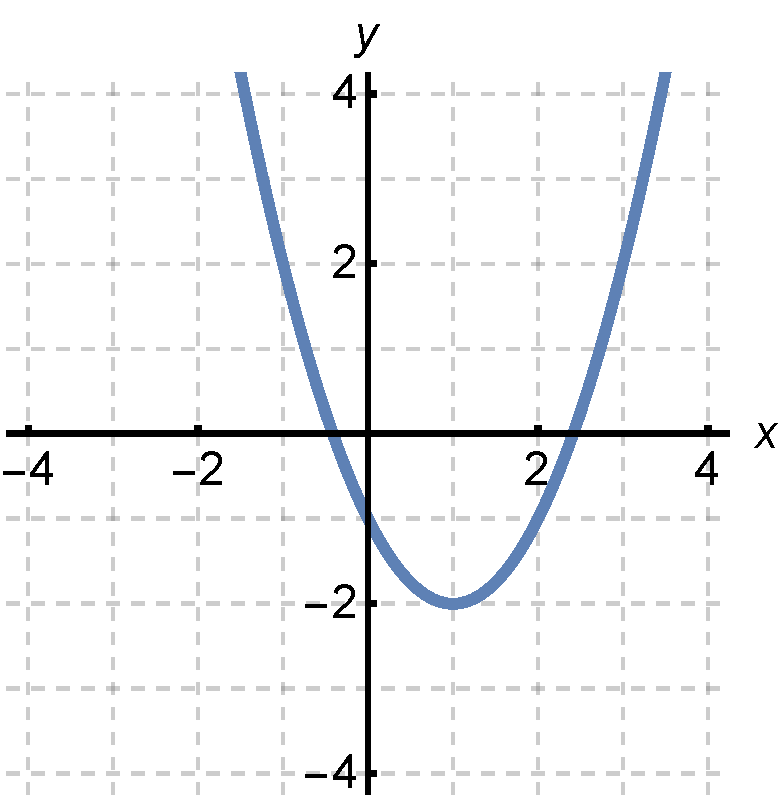
\includegraphics[valign=t,width=4.5cm]{parab}

\hrule
\smallskip
\hrule
%%

\begin{minipage}[t][][c]{0.5\textwidth}

\bigskip

(a) $$\begin{array}{|c|c|c|c|c|} \hline
x  & \hspace{.2in} & \hspace{.2in} & \hspace{.2in} & \hspace{.2in} \\ \hline
f(x)-2 &   &  &  &   \\
\hline
\end{array}$$

\end{minipage} \hfill \includegraphics[valign=t,width=4.5cm]{blank}


\hrule
%%

\begin{minipage}[t][][c]{0.5\textwidth}

\bigskip

(b) $$\begin{array}{|c|c|c|c|c|} \hline
x  & \hspace{.2in} & \hspace{.2in} & \hspace{.2in} & \hspace{.2in} \\ \hline
f(x-2) &   &  &  &   \\
\hline
\end{array}$$

\end{minipage} \hfill \includegraphics[valign=t,width=4.5cm]{blank}

\hrule
%

\begin{minipage}[t][][c]{0.5\textwidth}
	
	(c) $$\begin{array}{|c|c|c|c|c|} \hline
	x  & \hspace{.2in} & \hspace{.2in} & \hspace{.2in} & \hspace{.2in} \\ \hline
	-f(2x) &   &  &  &   \\
	\hline
	\end{array}$$	
	
\end{minipage} \hfill \includegraphics[valign=t,width=4.5cm]{blank}


\hrule
%

\begin{minipage}[t][][c]{0.5\textwidth}
	\medskip
	
	%Note to instructors: this next part is HARD for students. Remember, it's really helpful to point out that vertical transformations are achieved by doing an operation to the output, while horizontal transformations are achieved by replacing the input variable (which is not just the "stuff in parentheses", but x alone in these cases) by some something new.
	%
	%So e.g. here the first function is f(x) -> f(x+3) -> f((1/2)x + 3)
	%
	%while the second is f(x) -> f((1/2)x) -> f((1/2)(x+3))
	
 Consider $f(x)$ above.  First, shift left by 3, then make the graph wider by a factor of 2.  Sketch this function, and write down a formula for it in terms of $f$.
	\vskip2ex
	Now, start again, but this time, first make the graph wider by a factor of 2, then shift left by 3.  Again, sketch it and find a formula.  Is it the same function that you got previously?
	
	
\end{minipage} \hfill \includegraphics[valign=t,width=4.5cm]{blank}

\vspace*{-1cm}
\newpage


%
%Note to instructors: ask for or give them the algebraic definitions of even/odd here and connect them to reflections -- students tend not to see this connection to the symmetry they can see
%
\textbf{Even and odd functions}
\vskip2ex
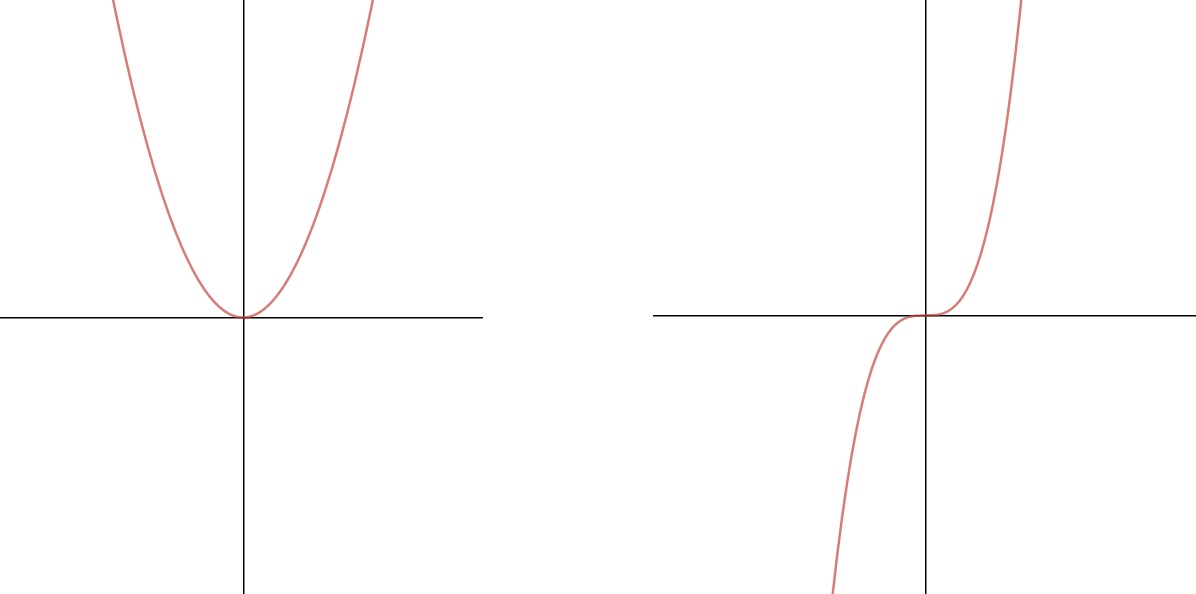
\includegraphics[width=2.5in]{evenodd.jpg}

\textbf{Inverse Functions}
	\begin{enumerate}
	
	\item If a function $f$ is invertible, its inverse is defined as follows: $$f^{-1}(y) = x \quad \textrm{means} \quad \underline{\hspace*{1.5in}}$$
	
	For the following graph, estimate $f^{-1}(0)$ and $f^{-1}(2)$, and sketch $f^{-1}$.
	

	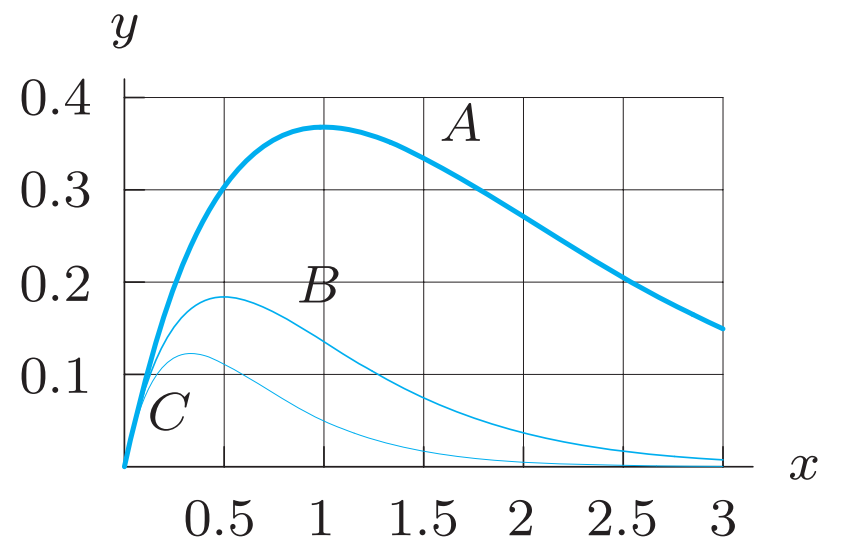
\includegraphics[width=3in]{graph.jpg}
	
	For the following table, find $f(2)$, $f^{-1}(2)$ and $f^{-1}(4)$.
	
	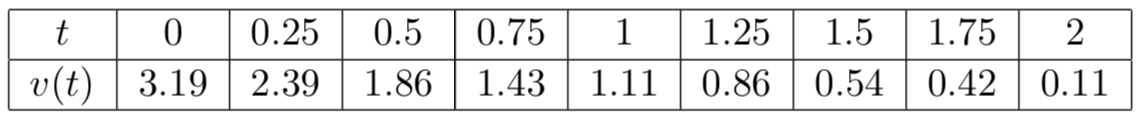
\includegraphics[width=3in]{table.jpg}
	\item Sketch graphs for the heights of a skydiver and a bungee jumper respectively.  Are they invertible?
	
	\vskip15ex
	A function has an inverse if and only if:
	\vskip5ex 
	
	
	\item Is $y=f(x) = 3x-5$ invertible?  If so, find the inverse.
	
	
	
	\newpage
	
	\item (1.3 \#19)
	
	
	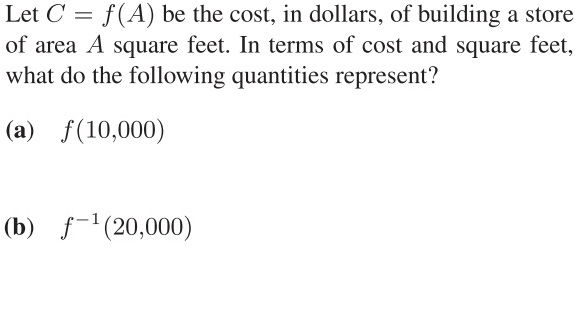
\includegraphics[width=3.5in]{no19.jpg}
	
	\textbf{Function Composition}
	\item (1.3 \#9) Let $f(x) = \sqrt{x+4}$ and $g(x) = x^2$.  Find 	$f(g(x))$ and 
	$g(f(x))$.

	\vskip10ex 
	\item (1.3 \#48--51)
	
	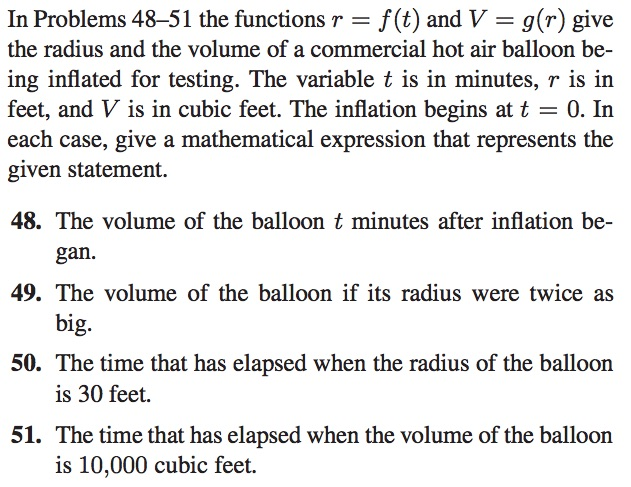
\includegraphics[width=4in]{no48.jpg}
	

	\end{enumerate}

\vfill
\textit{Extra practice}: 1.3 \#21, 31, 33, 45, 57, 59

\end{document}

